\def\year{2015}
%File: formatting-instruction.tex
\documentclass[letterpaper]{article}

% Required Packages
\usepackage{aaai}
\usepackage{times}
\usepackage{helvet}
\usepackage{courier}
\usepackage{mathtools}
\usepackage{breqn}
\usepackage{amsmath}
\usepackage{algorithm}
\usepackage[noend]{algpseudocode}
\def\BState{\State\hskip-\ALG@thistlm}
\frenchspacing
\setlength{\pdfpagewidth}{8.5in}
\setlength{\pdfpageheight}{11in}

% Section numbers. 
\setcounter{secnumdepth}{2}  

\nocopyright
\begin{document}
% Title and author information
\title{MatLab Simulation of a Rao-Blackwellized Particle Filter with Improved Techniques for Grid Mapping in Mobile robots}
\author{Adrian Llopart \\ P.h.D, DTU }
\maketitle


\begin{abstract}
\iffalse
A short summary of the paper and its main results/insights. Should preferably
be less than 150 words.
\fi
Rao-Blackwellized Particle filters have been introduced in simultaneous localization and mapping (SLAM) effectively in the past years. Improved techniques have helped reduce the number of particles needed and allowed a faster and more robust solution. These solutions can be seen, and used, in the C++ ROS \textit{gmapping} package. This paper presents the conversion to a simpler but easy-to-understand MatLab implementation and will describe the RBPF-SLAM principle in a similar manner.

\end{abstract}

\section{Introduction}
\iffalse
What problem are you trying to solve? Why is this important? What
are the main results/accomplishments/highlights of the paper. Since the reader is
assumed to be familiar with the details and goal of the programming project, this
section will probably be fairly short. But you can use it to briefly describe the type of
solution you have chosen and why.
\fi
One of the clearest functionalities of mobile robots is building maps of its surroundings and navigating through them; this is often referred to as SLAM, Simultaneous Localization and Mapping. There exists, however, certain difficulties when implementing SLAM, mainly, for a robot to localize (know its true position), a very precise map has to be built before; but, for a very precise map to be built, a robot must know exactly where it is. Friction, control loss or small obstacles are often the cause of a bad odometry which leads to a poor estimate of the true position. The Rao-Blackwellized Particle filter (as shown in ~\cite{Doucet} and ~\cite{Murphy}) solves this issue by generating estimates of the possible position (particles) and giving them a weight. Those particles that have a higher weight, because their estimate matches better the reality, will survive, and the rest will die out in the next generation. To keep a continuous amount of particles and not let all of them die out, resampling stages are carried out where those surviving particles reproduce and keep the particle count constant. It is evident that the more particles used, the more possible descriptions of the reality one has and the higher probability of having at least one particle which is almost perfect. This also induces a higher computational necessity and stops the solution from becoming a real-time application.\\
The real issue is therefore weighing these particles to know how close they are to the reality. This is known as the \textit{proposal distribution}, and in the latter iterations of the RBPF-SLAM solution, optimal techniques have been developed to obtain a more accurate representation whilst keeping the particle count to a minimum.\\
In summary, what the RBPF-SLAM algorithm does is given an initial estimate of the true pose, it will use the high precision of a laser scan and the latest map generation and converge the estimate to the true position. This leads to a more accurate map representation and a considerable reduction in errors and number of particles.

\section{RBPF joint posterior}
As presented by ~\cite{Murphy}, the key idea of RBPF-SLAM is to estimate the joint posterior $p(x_{1:t},m|z_{1:t}, u_{1:t-1})$. In other words, the algorithm should compute the true (or as close as possible) position ($x$) of the robot and a map ($m$) for every iteration, given solely the laser scan data ($z$) and the odometry measurements ($u$). This posterior can be factorized as follows:

\begin{multline}
p(x_{1:t},m|z_{1:t}, u_{1:t-1}) = \\ p(m|x_{1:t},z_{1:t}) \cdot p(x_{1:t}|z_{1:t}, u_{1:t-1})
\end{multline}

This allows us to estimate the position of the robot using the logged odometry and the laser scan data, and then use this position and the laser data again to generate more parts of the map. Thus, the generated map depends heavily on the estimate of the position. This technique is known as Rao-Blackwellization.
\subsection{Posterior over maps}
The posterior over maps ($p(m|x_{1:t},z_{1:t})$) can be computed analytically using several methods. This paper used the approach presented by ~\cite{ProbabilisticRobotics} known as \textit{Occupancy grid mapping} (Algorithm \ref{OGM}) and the \textit{Inverse sensor model} (pages 284-292) to generate a 2-D floor plan occupancy grid map.\\
Therefore, a map \textit{m} is partitioned into finitely many grid cells $m = {m_i}$, where each cell contains a value that refers to the probability of it being occupied ($p(m_i)$) with values ranging from '0' (free) to '1' (fully occupied). The posterior over maps can then be approximated as the product of its marginals.
\begin{equation*} 
p(m|x_{1:t},z_{1:t}) = \prod_{i} p(m_i|x_{1:t},z_{1:t})
\end{equation*}
It is worth noting that this algorithm will use the \textit{log-odds} representation of occupancy to avoid numerical instabilities for probabilities close to zero or one:
\begin{equation*} 
l_{t,i}= log \frac{p(m_i | z_{1:t}, x_{1:t})}{1-p(m_i | z_{1:t}, x_{1:t})}
\end{equation*}
and that the probability ration can be easily recovered from the \textit{log-odds} ratio as:
\begin{equation*} 
p(m_i | z_{1:t}, x_{1:t})= 1- \frac{1}{1+exp(l_{t,i})}
\end{equation*}
Finally, the algorithm makes use of the variables $l_0$, $l_{occupied}$ and $l_{free}$ which can be adjusted as one pleases. The values applied for this simulation are 0.5, 1 and -1. Also, $\alpha$ makes reference to the average width of walls; and $\beta$ is the width of the sensor beam. Considering that the simulation uses one cell to represent 10$cm^2$, $\alpha$ is set to be equal to 2 (thus 20 cm) and $\beta$ will be equal to 0.1.

\begin{algorithm}
	\caption{Complete Occupancy Grid Mapping}\label{OGM}
	\begin{algorithmic}[1]
		\Procedure{Occupancy\_Grid\_Mapping ($l_{t-1,i}$, $x_t$, $z_t$)}{}
		\For {$\text{all cells } m_i $}
		\If {$ m_i \text{ in perceptual field of } z_t$}
		\State $l_{t,i} = l_{t-1,i} + \textbf{inverse\_range\_sensor\_model(}m_i, x_t, z_t\textbf{)}-l_0$
		\Else
		\State $l_{t,i} = l_{t-1,i}$
		\EndIf
		\EndFor 
		\Return {$l_{t,i}$}
		\EndProcedure
		\\
		\Procedure{Inverse\_Range\_Sensor\_Model ($m_i$, $x_t$, $z_t$)}{}
		\State {$\text{Let } x_i, y_i \text{be the center of mass of } m_i$}
		\State $r = \sqrt{(x_i - x)^2 + (y_i - y)^2}$
		\State $\phi = atan2(y_i - y, x_i - x) - \theta$
		\State $k = argmin_j|\phi - \theta_{j, sens}|$
		\If {$r > min(z_{max}, z_t^k + \alpha /2) or |\phi - \theta_{j, sens}> \beta /2|$}
		\Return $l_0$
		\EndIf
		\If {$z_t^k  > z_{max} and |r-z_t^k|<\alpha /2$}
		\Return $l_{occupied}$
		\EndIf
		\If {$r \leq z_t^k $}
		\Return $l_{free}$
		\EndIf
		\EndProcedure
	\end{algorithmic}
\end{algorithm}

\subsection{Posterior over potential trajectories}
The posterior over potential trajectories $p(x_{1:t}|z_{1:t}, u_{1:t-1}$ will be solved applying a particle filter. This means that one particle will represent one potential trajectory over one time step and will also generate its own map.\\
Usually, a non-optimal particle filter called SIR (sampling importance resampling) is applied. this filter follows 4 main steps:
\begin{itemize}
	\item \textit{Sampling}: The next generation of particles $x_t^{(i)}$ is obtained from the previous generation $x_{t-1}^{(i)}$ by sampling form the proposal distribution $\pi$. Normally, a probabilistic odometry motion model is used here.
	\item \textit{Importance weighing}: each particle is assigned with a weight $w_t^{(i)}$ according to the importance sampling principle:
	\begin{equation}
		w_t^{(i)}=\frac{p(x_{1:t}^{(i)}|z_{1:t}, u_{1:t-1})}{\pi(x_{1:t}^{(i)}|z_{1:t}, u_{1:t-1})}
	\end{equation}
	which incorporates all observations and positions up until that specific point in time.
	\item \textit{Resampling}: New particles are drawn which replace the old ones depending on their weight. This keeps the particle count constant. the new generation of particles have all the same initial weight.
	\item \textit{Map estimation}: for every particle, a map is generated according to the approach presented before (Algorithm \ref{OGM}).
\end{itemize}
One might rapidly notice that this filter requires a trajectory weight evaluation after every observation/time step. hence, this schema becomes highly inefficient over time as trajectories grow. \cite{Weights}  obtained a recursive formulation to compute the importance weights, which allows the calculation of the next weight based on the previous one (and not having to calculate over and over again all weights until that point):
\begin{equation}
\label{recursiveweights}
	w_t^{(i)}= \frac{p(z_t|m_{t-1}^{(i)}, x_t^{(i)})p(x_t^{(i)}|x_{t-1}^{(i)}, u_{t-1})}{\pi(x_t | x_{1:t-1}^{(i)}, z_{1:t},u_{1:t-1})} \cdot w_{t-1}^{(i)}
\end{equation}
Generic particle particle filters rely heavily on the recursive structure of equation \ref{recursiveweights}, whilst leaving open what the proposal distribution will be and when the resampling should take place. This paper will focus on the improved techniques presented in \cite{Cyrill} to obtain an optimal proposal distribution based on both odometry and sensor data.

\section{RBPF Improved proposal}
As described previously, one needs to draw particles from the proposal distribution $\pi$ to obtain an estimate on the next generation of particles. logically, the more accurate the proposal is, the better the end result of the estimation. typically, particle filters use the odometry proposal distribution because it is easily computed and replacing said odometry distribution in equation \ref{recursiveweights} yields a very simple weight calculation:
\begin{equation}
w_t^{(i)}= p(z_t|m_{t-1}^{(i)}, x_t^{(i)}) \cdot w_{t-1}^{(i)}
\end{equation}
However, this approach leads to a suboptimal result. Specifically because the precision of the laser scan data is not taken into account. In other words, if we only sample from the odometry proposal, the importance weights between particles will end up differing significantly because the drawn samples only cover a fraction of the state space region, as shown in Figure \ref{odometry_motion_model}. If the laser scan data was incorporated, and knowing that it provides a very pinpointed area of high likelihood, the resulting estimation would be significantly more precise.  
\begin{figure}[h]
	\centering
	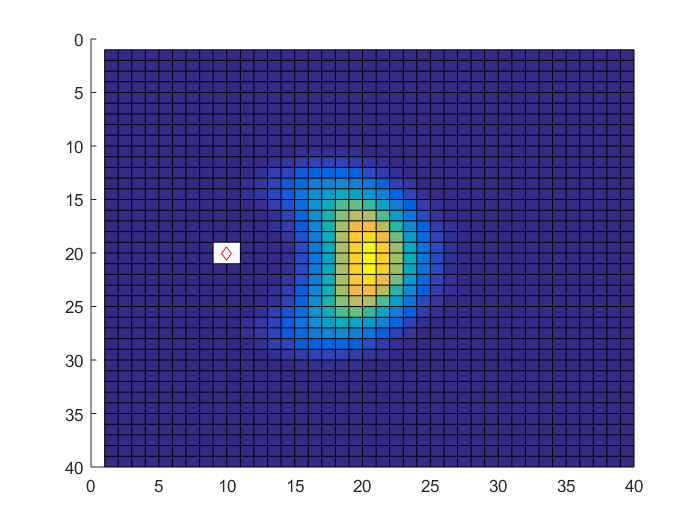
\includegraphics[width=0.5\textwidth]{figures/motion_model_odometry}
	\caption{Odometry proposal distribution for a 1 meter command}
	\label{odometry_motion_model}
\end{figure}
Therefore, integrating the sensor data $z_t$ into the proposal will focus the sampling only in the meaningful regions of the observation likelihood. The resulting distribution, according to \cite{optimal_proposal} is as follows: 
\begin{equation}
	\label{improved_proposal}
	p(x_t|x_{t-1}^{(i)}, m^{(i)}, z_t, u_t)=\frac{p(z_t|x_t, m^{(i)})p(x_t|x_{t-1}^{(i)}, u_t)}{p(z_t|x_{t-1}^{(i)}, m^{(i)}, u_t)}
\end{equation}
It is common practice to redefine the target distribution in equation \ref{improved_proposal} as:
\begin{equation*}
\tau (x_t)= p(z_t|x_t, m^{(i)})p(x_t|x_{t-1}^{(i)}, u_t)
\end{equation*} 

The major problem this approach has with grid maps is that the closed-form approximation of the proposal is not available due to an unpredictable shape of the observation likelihood function.\\ This could be solve applying an \textit{adaptive} particle filter which samples potential poses $x_j$ from the motion model and then weights them through the observation likelihood to obtain an approximation of the optimal proposal. Since the observation likelihood is typically peaked in very small areas, a dense sampling is necessary to capture correctly the peak, leading to a sub-optimal proposal, much like the motion model, because of its high computational requirements. Thus this paper will not pursue this approach.\\
Another way of solving this major issue is by taking into consideration that the observation likelihood typically has only one maxima allowing us to sample around this maxima and avoiding other less meaningful regions. Specifically, the posterior $p(x_t|x_{t-1}^{(i)}, m^{(i)}, z_t, u_t)$ is locally approximated around the maxima of the observation likelihood via a \textit{scan matching} procedure. 

\subsection{Scan matching approach}
This approach has a series of steps:\\
Initially, the next generation of particles is sampled from the odometry distribution. These particles are then approximated to the meaningful area of the observation likelihood via a \textit{Scan matching} method. In this process, the current scan data $z_t$ is compared to the particle´s map generated up until this point $m_i$ to converge the initial guess of the particles position to one that is closer to the reality. The algorithm used in this paper is known as ICP (Iterative Closest Point) which returns translational and rotational vectors that are applied to $x_t$ to reach a better position estimate. The algorithm takes into account two sets of point clouds and iteratively overlays them by minimizing the squares error.\\
We now want to sample around this new estimated position. To do so, first a Gaussian has to be determined around it. To calculate the mean $\mu^{(i)}$ and the variance $\Sigma^{(i)}$ we also take into account the odometry information:
\begin{equation}
\label{mu}
\mu^{(i)}= \frac{1}{\eta^{(i)}}\cdot \sum_{j=1}^K x_j \cdot p(z_t|m_{t-1}^{(i)}, x_j) \cdot p(x_j|x_{t-1}^{(i)}, u_{t-1})
\end{equation} 
\begin{multline}
\label{sigma}
 \Sigma_t^{(i)}= \frac{1}{\eta^{(i)}}\cdot \sum_{j=1}^K p(z_t|m_{t-1}^{(i)}, x_j) \cdot p(x_j|x_{t-1}^{(i)}, u_{t-1}) \\ \cdot (x_j - \mu_t^{(i)})(x_j - \mu_t^{(i)})^T 
\end{multline} 
with the normalization factor:
\begin{multline}
\eta^{(i)}= \sum_{j=1}^K p(z_t|m_{t-1}^{(i)}, x_j) \cdot p(x_j|x_{t-1}^{(i)}, u_{t-1}) =\sum_{j=1}^K \tau (x_t)
\end{multline} 
Now we have a closed-form approximation of the optimal proposal. As shown in \cite{Cyrill}, using the new proposal distribution, the new weights are calculated as:
\begin{equation}
\label{Weights}
w_t^{(i)}=w_{t-1}^{(i)} \cdot \eta^{(i)} = w_{t-1}^{(i)} \cdot \sum_{j=1}^K \tau (x_t)
\end{equation} 


The main advantage of the improved proposal is that it takes both the odometry data and laser scans into consideration which reduces notably the proposals densities uncertainty and allows more efficient sampling. The only problem this approach presents is when the observation likelihood is multimodal. Since the scan matching algorithm maximizes the observation likelihood around the closest local maxima to the initial guess, it is possible that this approximation fails because it misses other additional maxima due to the multimodlity of the likelihood. In other words, the reported local maxima is not the global maxima. However, in reality, the distribution tends to be uni-modal, as reported in \cite{Cyrill}, and so this issue is of little concern in common practices.\\
Another problem is when the scan matcher fails to report a scan conversion. This is generally because of poor observations or low overlapping areas between scans. For this case in particular, the proposal will only be determined by the raw motion model. This issue, however, is, in reality, not very common.

\section{RBPF Adaptive resampling}

The second main difference, this paper presents, with other general particle filters concerns the resampling step. During resampling, particles with low weight are replaced by new ones with higher weight. This is essential because only a finite amount of particles are used to approximate the target distribution; but, if not applied carefully, the resampling can remove good samples and lead to impoverishment of the particle filter. Also, the criterion for deciding when to resample is of utmost importance for a good overall performance.\\
The approach used in this paper relies in the so-called effective sampling size for target posterior estimation \cite{Liu}. This value was proposed by \cite{Weights} to be:
\begin{equation}
N_{eff}= \frac{1}{\sum_{i=1}^N (\bar w^{(i)})^2}
\end{equation}
where $\bar w^{(i)}$ is the normalized weight of the particle $i$.\\
The key idea behind $N_{eff}$ is that the worse the particle approximation is, the larger variance between weights there would be.  If the estimate was perfect, all particles would end up with the same weight value. As presented in \cite{Cyrill}, the resampling step should carried out when the value of $N_{eff}$ drops below $N/2$, where $N$ is the total number of particles.

\section{The RBPF improved algorithm}
The algorithm \ref{RBPF-SLAM} presents the full schema for the improved RBPF utilized in this paper. The steps are as follows:
\begin{itemize}
	\item An initial estimate of each particles position $x_t^{(i)}$ is obtained from the previous pose $x_{t-1}^{(i)}$, the odometry measurements $u_{t-1}$ and a realistic approximation of the errors the odometry might propose.
	\item A scan matching algorithm, in this case an ICP, is executed between the latest laser scan data $z_t$ and a point cloud derived form the latest map generated for that particle. To calculate the point cloud from the map, only that area inside what would be the region of the laser scanner is evaluated. This saves important resources and does not calculate point clouds in regions that cannot be matched with the laser scan data. The rotational and translational vectors derived through the ICP are used to reconstruct a new pose estimate $\dot x_t^{(i)}$ from the motion model estimate $x_t^{(i)}$. Finally, if the scan matcher fails at converging both point clouds, the pose estimate will remain as the one obtained from the motion model
	\item A set of sampling points $x_j$ is selected in an interval around $\dot x_t^{(i)}$. The mean and covariance values for creating a Gaussian distribution are calculated as in equations \ref{mu} and \ref{sigma} via a pointwise evaluation of the target proposal. The first half of the target proposal,  $p(x_j|x_{t-1}^{(i)}, u_t)$, is obtained by evaluating the sample $x_j$ in the odometry motion model distribution. The second half of the target distribution, $p(z_t|x_j, m^{(i)})$, is obtained evaluating the observation likelihood for that sample. Several approaches can be taken; this paper has used a point to point comparison between the true scan and the estimated scan a robot in the estimated position in the generated map would see. In this stage the weighing factor $\eta^{(i)}$ is also computed. 
	\item A new final pose estimate for particle $(i)$ is drawn from the Gaussian approximation $\mathcal{N} (\mu_t^{(i)}, \Sigma_t^{(i)})$ of the improved proposal.
	\item Update importance weights as in equation \ref{Weights}
	\item The particles map $m_i$ is updated with the final estimated position $\dot x_t^{(i)}$ and the laser scan data $z_t$.
	\item The resampling stage is carried out depending on the value of $N_{eff}$.
\end{itemize}

\begin{algorithm}
	\caption{Improved techniques for RBPF in grid mapping}\label{RBPF-SLAM}
	\begin{algorithmic}[1]
		\Procedure{RBPF-SLAM ($x_{t-1}$, $z_t$, $u_t$, $m_{t-1}$)}{}
		\State $ \mathcal{S}_{t-1}: \text{sample set of the previous time step} $
		\For {$\mathcal{S}_{t-1}^{(i)} \in \mathcal{S}_{t-1}$}
		\State $ < x_{t-1}^{(i)}, w_{t-1}^{(i)}, m_{t-1}^{(i)} > = \mathcal{S}_{t-1}^{(i)}$
		\State $ \text{// initial pose estimate} $
		\State $ x_t^{(i)} = x_{t-1}^{(i)} \oplus u_t$
		\State $ \text{// scan matching}$
		\State $ \dot x_t^{(i)} = \text{argmax}_x p(x|m_{t-1}^{(i)}, z_t. x_t^{(i)})$
		\If {$dot x_t^{(i)}$ = failure}
		\State $ x_t^{(i)} \sim  p(x_t|x_{t-1}^{(i)}, u_{t-1})$
		\State $w_t^{(i)}=w_{t-1}^{(i)} \cdot p(z_t|x_t, m^{(i)}) $
		\Else
		\State $ \text{// sample around node} $ 
		\For {$k=1,...,K$}
		\State $ x_k \sim \left\{ x_j || x_j - \dot x_t^{(i)}| < \Delta \right\} $
		\EndFor
		\State $ \text{// compute gaussian}$
		\For {all $ x_j \in \left\{ x_1,...,x_K \right\} $}
		\State $ \mu_t^{(i)}  = \mu_t^{(i)} + x_j \cdot p(z_t|m_{t-1}^{(i)}, x_j) \cdot p(x_j|x_{t-1}^{(i)}, u_{t-1})$
		\State $ \eta^{(i)}  = \eta^{(i)} + p(z_t|m_{t-1}^{(i)}, x_j) \cdot p(x_j|x_{t-1}^{(i)}, u_{t-1})$
		\EndFor
		\State $\mu_t^{(i)}  = \mu_t^{(i)} / \eta^{(i)} $
		\State $ \Sigma_t^{(i)}=0$
		\For {all $ x_j \in \left\{ x_1,...,x_K \right\} $}
		\State $ \Sigma_t^{(i)}= \Sigma_t^{(i)} + p(z_t|m_{t-1}^{(i)}, x_j) \cdot p(x_j|x_{t-1}^{(i)}, u_{t-1}) \cdot (x_j - \mu_t^{(i)})(x_j - \mu_t^{(i)})^T  $
		\EndFor
		\State $ \Sigma_t^{(i)}= \Sigma_t^{(i)}/ \eta*{(i)}$
		\State $ \text{// sample new pose from gaussian}$
		\State $ x_t^{(i)} \sim \mathcal{N} (\mu_t^{(i)}, \Sigma_t^{(i)}) $
		\State $ \text{// update importance weights}$
		\State $ w_t^{(i)}=w_{t-1}^{(i)} \cdot \eta^{(i)} $
		\EndIf
		\State $ \text{// update map}$
		\State $ m_t^{(i)} = \text{Occupancy\_Grid\_Mapping} (m_{t-1}^{(i)}, x_t, z_t)$
		\State $ \text{// update sample set}$
		\State $ \mathcal{S}_t = \mathcal{S}_t \cup  \left\{ < x_{t-1}^{(i)}, w_{t-1}^{(i)}, m_{t-1}^{(i)} > \right\} $
		\EndFor
		\State $ N_{eff} = \frac{1}{\sum_{i=1}^N (\bar w^{(i)})^2} $
		\If {$ N_{eff} < N/2$}
		\State $\mathcal{S}_t = <text{resample} \mathcal{S}_t $
		\EndIf
		\EndProcedure
	\end{algorithmic}
\end{algorithm}

\section{Simulations and results}
The  \textit{Matlab} code to which this paper refers to works with a simulated RBPF-SLAM. The user is able to create its own map (Figure \ref{initial_map}), generate a path which the robot should follow, adjust a series of parameters related to the motion model of the robot or related to the particle filter itself, and simulate the results for a RBPF-SLAM (Figure \ref{end_map}).

\begin{figure}[h]
	\centering
	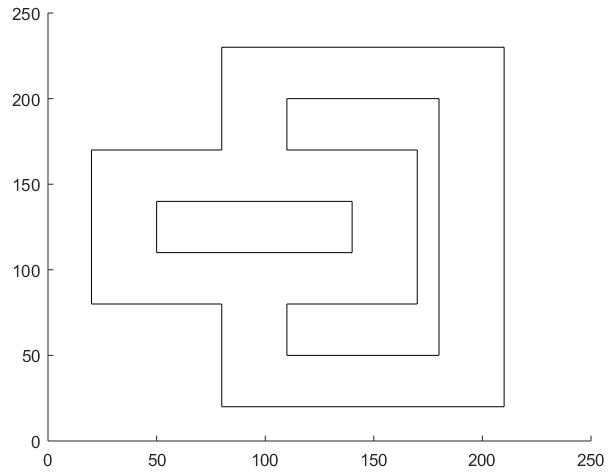
\includegraphics[width=0.4\textwidth]{figures/initial_map}
	\caption{Map created by the user}
	\label{initial_map}
\end{figure}
\begin{figure}[h]
	\centering
	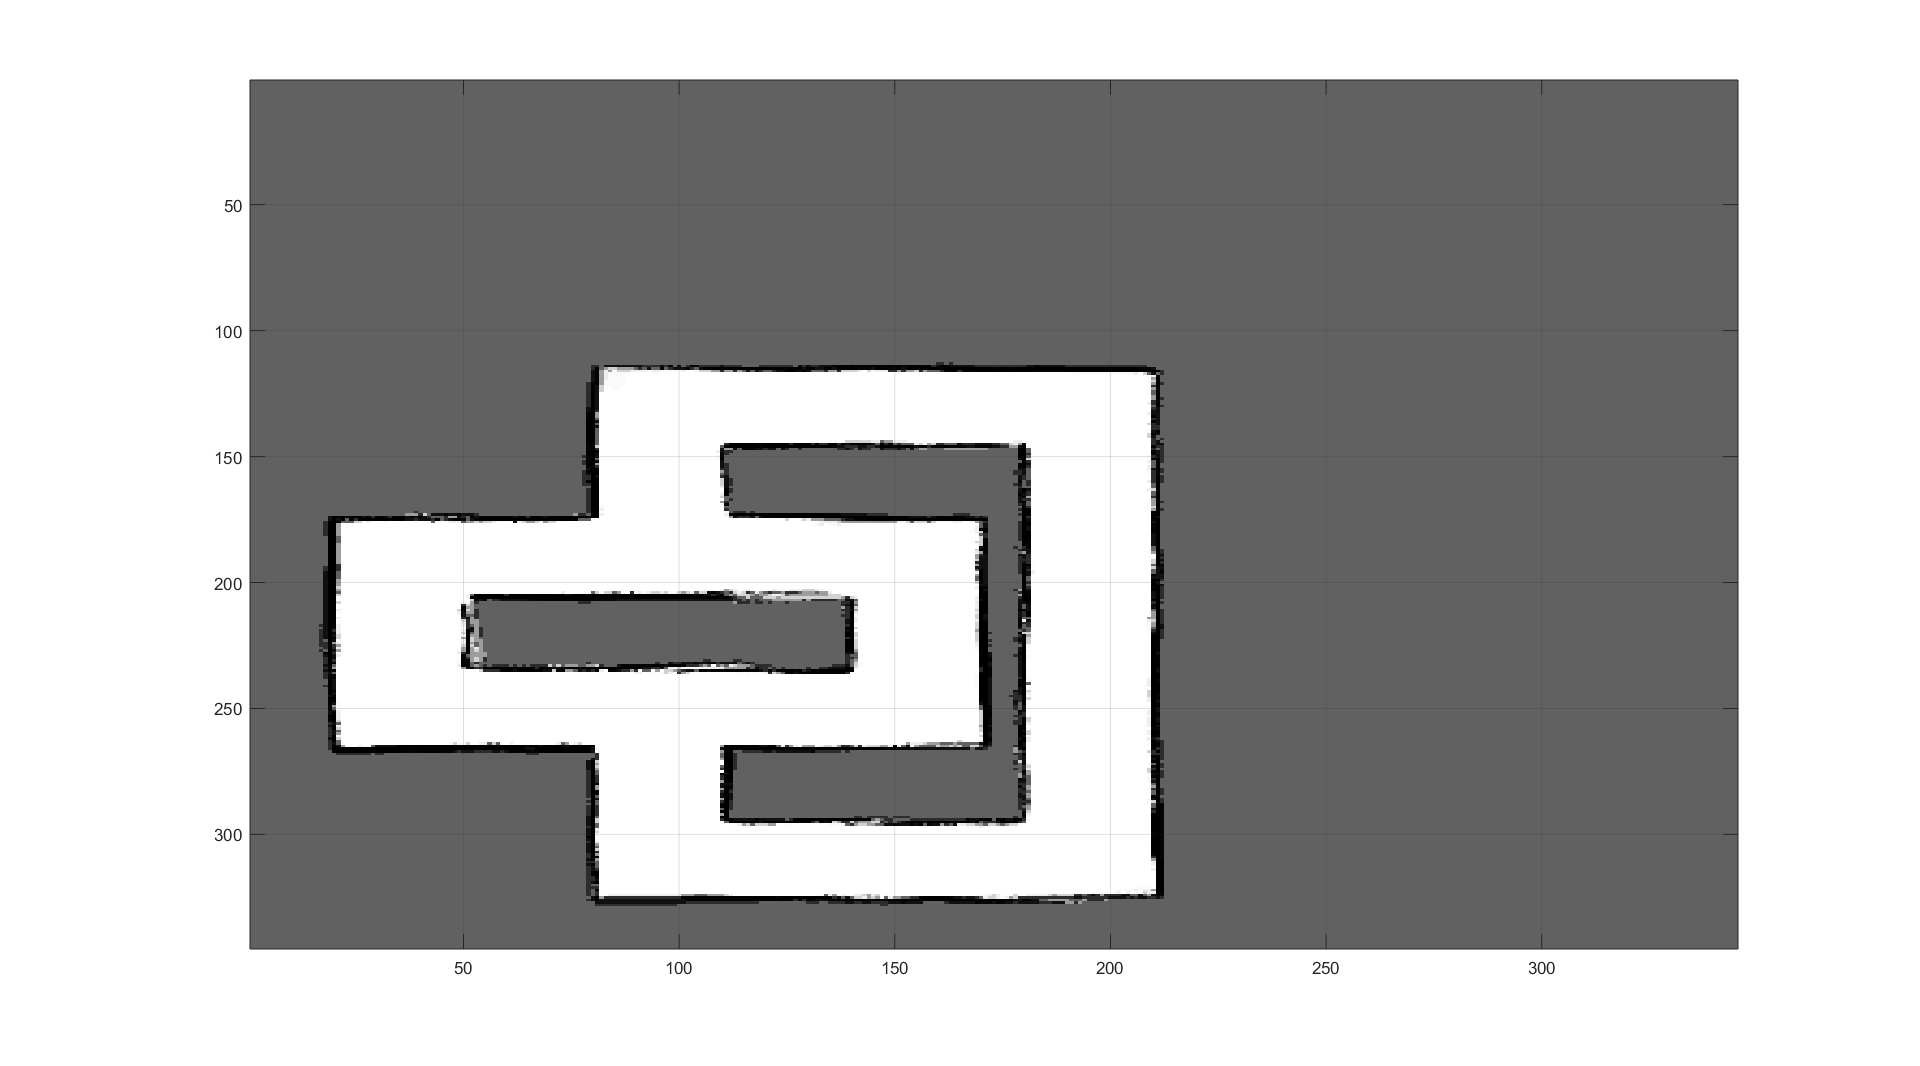
\includegraphics[width=0.37\textwidth]{figures/end_map}
	\caption{occupancy grid map generated after running RBPF-SLAM}
	\label{end_map}
\end{figure}

The resulting grid map will have a resolution of 10$\frac{cm^2}{cell}$ \\

The errors generated via this schema can be seen in Figure \ref{error_estimation}. They are minimal except for a particular point in which \textit{theta} overshoots. This is definitely due to misalignments in \textit{theta} for the case $0^o = 360^o$.

\begin{figure}[h]
	\centering
	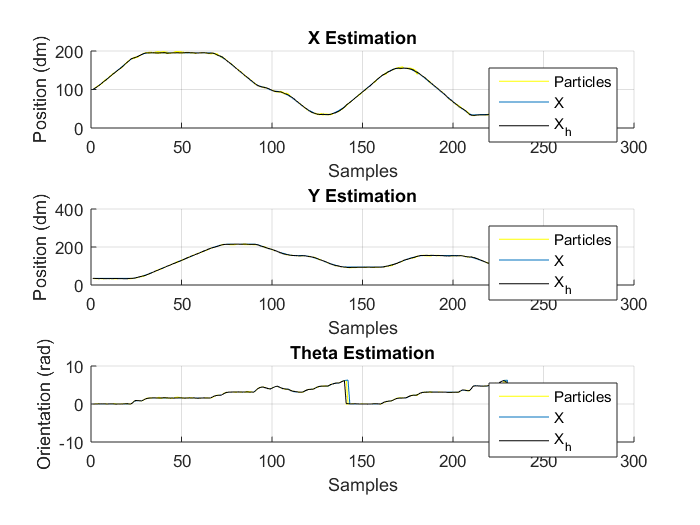
\includegraphics[width=0.37\textwidth]{figures/error_estimation}
	\caption{Error between the real and estimated \textit{x}, \textit{y} and \textit{theta} values}
	\label{error_estimation}
\end{figure}

% References and end of paper
\bibliographystyle{aaai}
\bibliography{bibliography}

\end{document}
